
\chapter{Design and Implementation}
\label{cha:design_and_implementation}

During the design and development of the  library one of the goals was for it to be totally independent and self-contained. The method was planed to be used together with SVO but it had to be independent from it. For this reason non of the classes and data structures defined in SVO has been used during the implementation, only third-party libraries openly available to everybody.\\

This definition leaded to have some redundant definitions because in the end, this method is using a subset of the data from SVO. For example, the class SVO::Frame and the class reloc::Frame are somehow similar.\\

Different methods have been developed here, an interface has been created to be able to used one or an other dynamically at run time. The interface is the abstract class reloc::AbstractRelocalizer, a pointer of this class is initialized to point to the real relocalizer algorithm. It can be then used transparently with no knowledge of the implementation is.\\

The interface has been created with the following important methods:

\begin{itemize}
  \item \textit{addFrame}: This method is used to add a new frame used to relocalize, usually only keyframes are added to the relocalizer.
 
  \item \textit{removeFrame}:  Sometimes, a frame should not be used any more, for instance, when the vehicle is sure it has moved to a different area.

  \item \textit{train}: Some of the implemented methods need to train before it is able to relocalize. It should always be executed, but not all methods will do something.

  \item \textit{relocalize}: This is the actual method used when the vehicle is lost. Given one new image, it will try to find its current 6 DoF pose.
\end{itemize}

There are two implementations of the interface as can be seen in~\ref{fig:abstract_classreloc}. \textit{MultipleRelocalizer} implement the two problems, Place Finder and Real Pose Finder, and connects them. Interfaces to solve those problems have been implemented too, so this class only contains pointers to its abstract interface. Different solutions can be used and are interchangeable. \\

\begin{figure}[htpb]
  \centering
  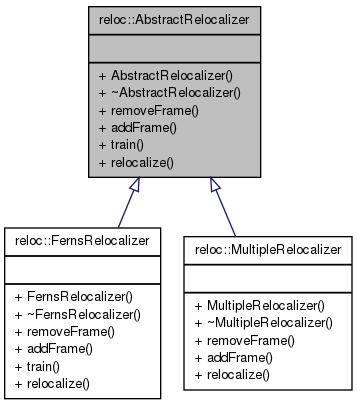
\includegraphics[width=6cm]{img/class_abstractreloc.png}
  \caption{Relocalizer class interface and implementations}
  \label{fig:abstract_classreloc}
\end{figure}

The \test{Place Finder} interface has two important methods:

\begin{itemize}
  \item \textit{add/removeFrame}: The methods from the \textit{relocalizer} with the same name pass its arguments to this methods. Here is where actual computation might be performed depending on the implementation.
  \item \textit{findPlace}: This method tries to find the closes stored frame to the query image.
\end{itemize}


Only one implementation is available at the moment, using the cross correlation estimation similarly to the PTAM method. In~\ref{fig:class_abstract_placerecognition} a second implementation can be seen, it uses the actual known pose of frames. It can only be used when is information is available, which is only when testing with known ground truth. It will always find the best option available, and it is used to test different \textit{Real Pose Finder} implementations when this first step is optimal. \\

\begin{figure}[htpb]
  \centering
  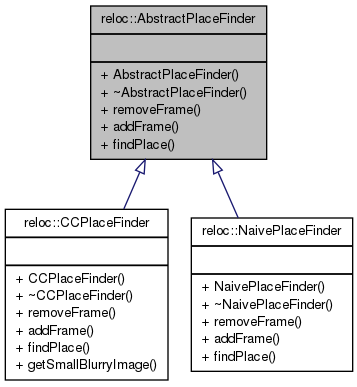
\includegraphics[width=6cm]{img/class_abstract_placerecognition.png}
  \caption{Place Finder interface and implementations}
  \label{fig:class_abstract_placerecognition}
\end{figure}

\begin{figure}[htpb]
  \centering
  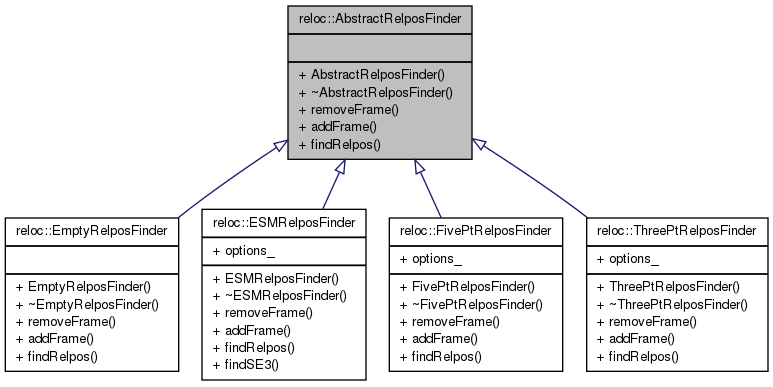
\includegraphics[width=9cm]{img/class_abstract_relposfinder.png}
  \caption{Real Pose Finder interface and implementations}
  \label{fig:class_abstract_relposfinder}
\end{figure}

Finally, there is also an interface for \textit{Real Pose Finder}, it can be seen in Figure~\ref{fig:class_abstract_relposfinder} along with all its implementations. The methods follow the same idea as for \textit{Place Finder} except for one method:

\begin{itemize}
  \item \textit{findRelps}: this method computes the transformation between two frames. The frame found by \textit{Place Finder} and the new frame are used as input.
\end{itemize}


A class have been created to contain all the information from a frame that might be needed in the different processes, it eases the propagation of information. Also, the use of smart pointers on it eases the memory management and the data redundancy. The class reloc::Frame has the next information:

\begin{itemize}
  \item \textbf{Image Pyramid}: A list of different scales of the same image.
  \item \textbf{Transformation World to Frame}: The $SE(3)$ transformation from the world frame to the camera frame when the image was taken.
  \item \textbf{Features}: A list of salient points in the image. Every feature contains:
    \begin{itemize}
      \item The image point where it was found
      \item The pyramid scale level where it was found
      \item If known, the world frame point to which it corresponds
    \end{itemize}
\end{itemize}

\section{Third-party libraries}
\label{sec:third_party_libraries}

Those libraries have been used and are third-party dependencies:

\begin{itemize}
  \item \textbf{OpenCV}: Mostly for its image encapsulation. Also used in image warping and descriptor extraction

  \item \textbf{Eigen}: General matrix operations and linear algebra solutions

  \item \textbf{Sophus}: Lie algebra groups implementation using Eigen

  \item \textbf{OpenGV}: Three point algorithm implementation using Eigen
\end{itemize}

